\section{Validation of the model}
For the last set of tests, we returned over the initial optical bench. In this case, we wanted to compare the output of the model with the resolution of the camera, in order to understand if the precision of the measures we can make, is inferiorly limited by camera resolution, or if it is influenced also by some other factors. \\
To reach our goal, we decided to modify the bench a bit: we used a less distorted lens (the one used in the Section \ref{sec:exp1} introduced too much tangential distortion), and we changed the laser to a similar one to that used in Section \ref{sec:exp2}, less noisy and thick than the initial one (configuration in Table \ref{tab:conf3}). Thus, we calibrate the system again, using the company's software. At this point, we performed two different test:
 \begin{itemize}
   \item First, we repeated the experiments in Section \ref{sec:exp1}, using the same known target object.
   \item Second, we empirically evaluated the resolution of the camera, and compared the results with both the nominal value of the camera, and the results obtained in the first point.
 \end{itemize}
 \begin{table}
  \centering
  \begin{tabular}{ccccc}
  \hline
  \multicolumn{5}{|c|}{\textbf{Camera}}                                                                                                                                                                            \\ \hline
  \multicolumn{1}{|c|}{\textbf{Name}} & \multicolumn{1}{c|}{\textbf{Size}}      & \multicolumn{1}{c|}{\textbf{Pixel size}} & \multicolumn{1}{c|}{\textbf{Lens Manufacturer}} & \multicolumn{1}{c|}{\textbf{Focal}} \\ \hline
  \multicolumn{1}{|l|}{}              & \multicolumn{1}{c|}{\textit{pix x pix}} & \multicolumn{1}{c|}{\textit{mum}}        & \multicolumn{1}{c|}{}                           & \multicolumn{1}{c|}{\textit{mm}}    \\ \hline
  \multicolumn{1}{|l|}{Arya}          & \multicolumn{1}{c|}{4096 x 3072}        & \multicolumn{1}{c|}{5.5}                 & \multicolumn{1}{c|}{Shneider}                   & \multicolumn{1}{c|}{35}             \\ \hline
  \multicolumn{1}{l}{}                & \multicolumn{1}{l}{}                    & \multicolumn{1}{l}{}                     & \multicolumn{1}{l}{}                            & \multicolumn{1}{l}{}                \\ \cline{2-4}
  \multicolumn{1}{c|}{}               & \multicolumn{1}{c|}{\textbf{Laser}}     & \multicolumn{1}{c|}{}                    & \multicolumn{1}{c|}{}                           &                                     \\ \cline{2-4}
  \multicolumn{1}{c|}{}               & \multicolumn{1}{c|}{\textbf{Frequency}} & \multicolumn{1}{c|}{\textbf{Power}}      & \multicolumn{1}{c|}{\textbf{Aperture}}          &                                     \\ \cline{2-4}
  \multicolumn{1}{c|}{\textit{}}      & \multicolumn{1}{c|}{\textit{nm}}        & \multicolumn{1}{c|}{\textit{W}}          & \multicolumn{1}{c|}{\textit{degree}}            & \textit{}                           \\ \cline{2-4}
  \multicolumn{1}{c|}{}               & \multicolumn{1}{c|}{450}                & \multicolumn{1}{c|}{1.6}                 & \multicolumn{1}{c|}{45}                         &                                     \\ \cline{2-4}
  \end{tabular}

  \caption{Configuration of the third system.}
  \label{tab:conf3}
\end{table}

% --------- %
\subsection{Model validation}
In the first phase, the experiments were performed as described in Section \ref{sec:exp1}, but now we have limited the propagation of the errors to the single points, rather than proceeding with the measurements as before. Thus, we put the target in three know position: at the beginning, in the middle and at the end of the \acs{FOV}. This allowed us to cover the entire \acs{FOV} of the camera. In Table \ref{tab:exp3-res} we reported the obtained results. As before, the values are the means of the propagate error for each point over the same sub-filter. We repeated our analysis twice because, as we can see, in the first test, the target was taken in wrong positions. However, we reported all the results better to find some correlations with the results discussed in the next subsection. \\
  \begin{table}[b!]
\centering
\begin{tabular}{|l|l|r|r|r|l|l|l|l|}
\cline{1-1} \cline{3-5} \cline{7-9}
\multirow{3}{*}{} &  & \multicolumn{3}{c|}{\textbf{Test 1}}                                                                            &  & \multicolumn{3}{c|}{\textbf{Test 2}}                                                                            \\ \cline{3-5} \cline{7-9} 
                  &  & \multicolumn{1}{c|}{\textbf{Begin}} & \multicolumn{1}{c|}{\textbf{Center}} & \multicolumn{1}{c|}{\textbf{End}}  &  & \multicolumn{1}{c|}{\textbf{Begin}} & \multicolumn{1}{c|}{\textbf{Center}} & \multicolumn{1}{c|}{\textbf{End}}  \\ \cline{3-5} \cline{7-9} 
                  &  & \multicolumn{1}{c|}{\textit{(mm)}}  & \multicolumn{1}{c|}{\textit{(mm)}}   & \multicolumn{1}{c|}{\textit{(mm)}} &  & \multicolumn{1}{c|}{\textit{(mm)}}  & \multicolumn{1}{c|}{\textit{(mm)}}   & \multicolumn{1}{c|}{\textit{(mm)}} \\ \cline{1-1} \cline{3-5} \cline{7-9} 
\textbf{COM 16}   &  & 0.4320                              & 0.5635                               & 0.5915                             &  & 0.2997                              & 0.3211                               & 0.4247                             \\ \cline{1-1} \cline{3-5} \cline{7-9} 
\textbf{COM 20}   &  & 0.4322                              & 0.5638                               & 0.5910                             &  & 0.2798                              & 0.3212                               & 0.4247                             \\ \cline{1-1} \cline{3-5} \cline{7-9} 
\textbf{BR 16}    &  & 0.4322                              & 0.5642                               & 0.5917                             &  & 0.2800                              & 0.3216                               & 0.4251                             \\ \cline{1-1} \cline{3-5} \cline{7-9} 
\textbf{BR 20}    &  & 0.4322                              & 0.5644                               & 0.5636                             &  & 0.2800                              & 0.3217                               & 0.4251                             \\ \cline{1-1} \cline{3-5} \cline{7-9} 
\textbf{FIR}      &  & 0.4323                              & 0.5636                               & 0.5920                             &  & 0.2800                              & 0.3215                               & 0.4250                             \\ \cline{1-1} \cline{3-5} \cline{7-9} 
\end{tabular}
\caption{Error propagation to points, at the begin, the middle and the end of the \acs{FOV}}
\label{tab:exp3-res}
\end{table}
For the moment, the only consideration that we can make is the comparison with the results in Section \ref{sec:exp1}: the use of a less distorted lens, and the use of a better laser reduced significantly the theoretical error that we can commit.

% --------- %
\subsection{Camera resolution}
In the second phase, we decided to integrate our library with a method that allowed us to evaluate the resolution of the camera. To do that, we put the step motor, used to calibrate the system, parallel with the optical axis; in this way the reference object (used to create the grid of points required by Tsai) is perpendicular with the camera. In this case we are not interested in determining the edges of the object, but only to acquire a horizontal laser line. So, we saved six frames: two at the beginning of the \acs{FOV}, two in the middle, and two at the end; in each pair of the acquisitions, the laser lines are $5 \, mm$ apart. This value was chosen arbitrarily to appreciate the distance to the naked eye, and to be able to control the displacement between one position and the other with a tape measure. In Figure \ref{fig:line-pos} are shown the three positions of the target, with respect of the \acs{FOV} of the camera.
  \begin{figure}[!b]
    \centering
    \begin{minipage}[c]{.32\textwidth}
      \centering
      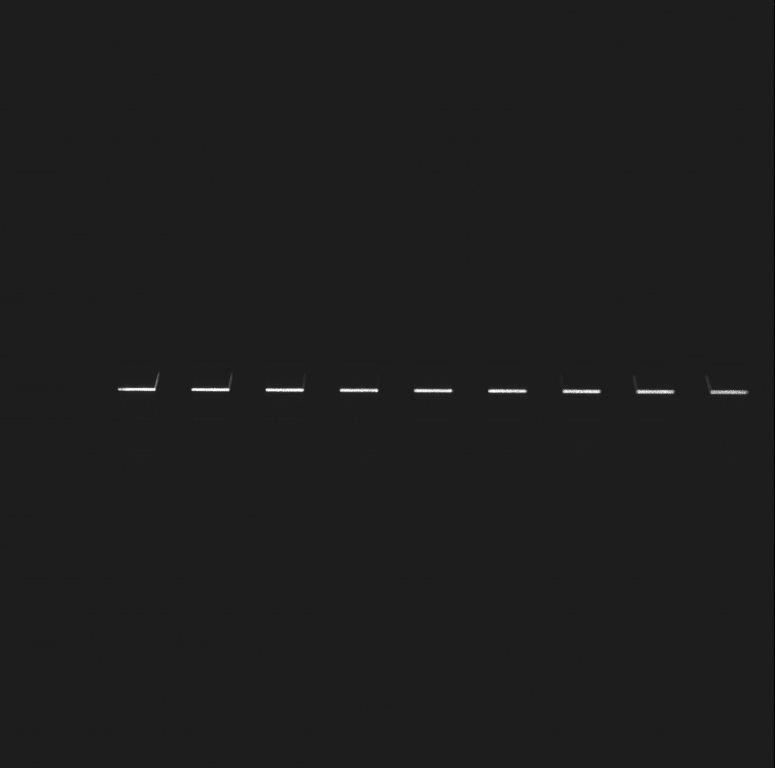
\includegraphics[width=\textwidth]{./images/analysis/exp3/250.jpg}
    \end{minipage}
    \hfill
    \begin{minipage}[c]{.32\textwidth}
      \centering
      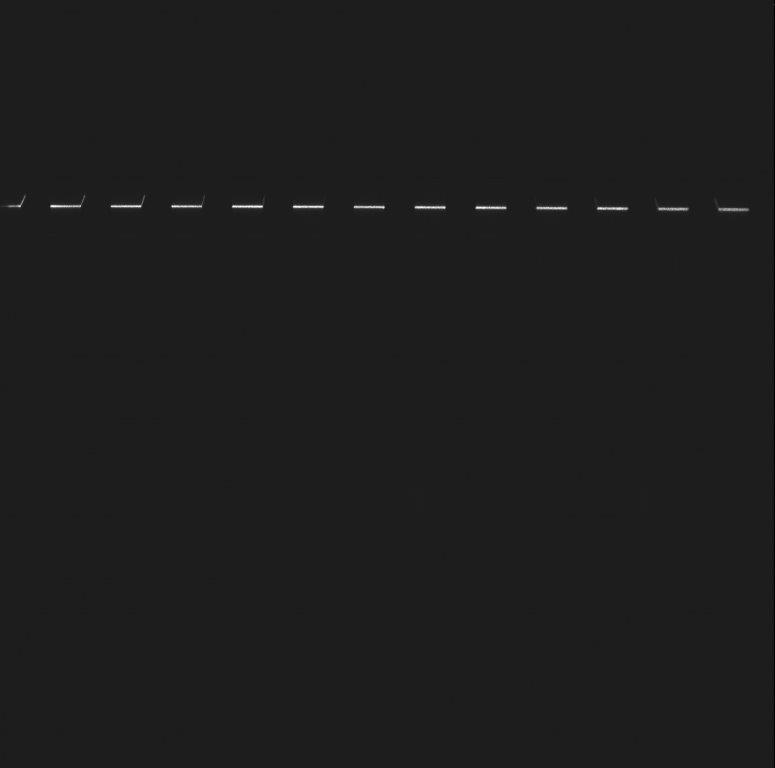
\includegraphics[width=\textwidth]{./images/analysis/exp3/380.jpg}
    \end{minipage}
    \hfill
    \begin{minipage}[c]{.32\textwidth}
      \centering
      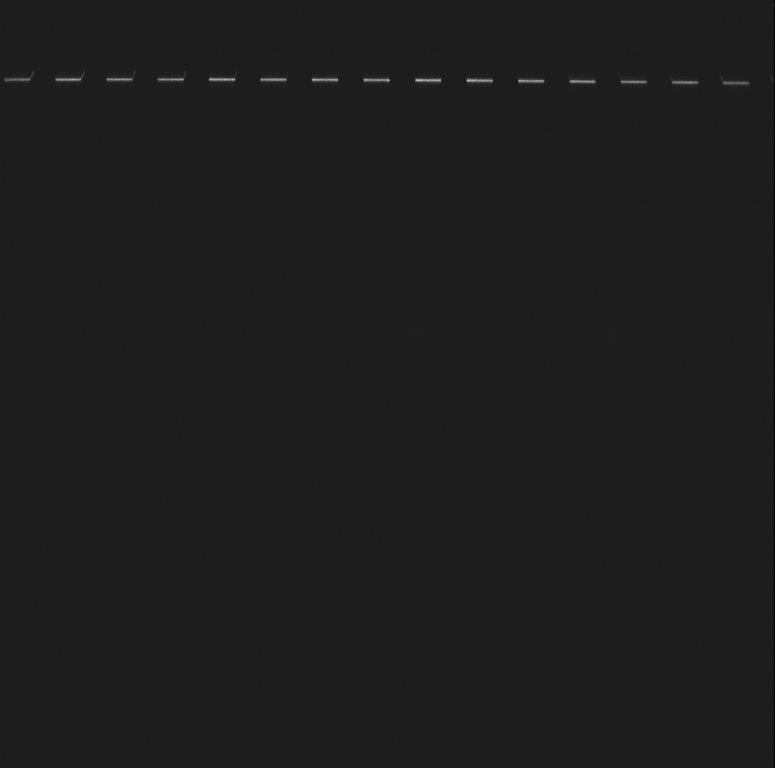
\includegraphics[width=\textwidth]{./images/analysis/exp3/510.jpg}
    \end{minipage}
    
    \caption{Positions of the target along the \acs{FOV} of the camera}
    \label{fig:line-pos}
  \end{figure}
In Table \ref{tab:exp3:res2} we reported our results: the first two columns are, respectively, the distances and the errors between the pairs of laser lines, while the third column contains the resolution of the camera, evaluated in the three position cited above. As we can see, the filters did not change resolutions substantially, so we can conclude that the resolution of our camera was in the range $\left( 0.27, 0.55 \right) \, mm/pix$. \\
  \begin{table}[t!]
  \centering
  \begin{tabular}{|cl|p{2.3cm}|p{2.3cm}|p{2.3cm}|}
  \hline
  \multicolumn{2}{|c|}{\multirow{2}{*}{}}              & \multicolumn{1}{c|}{\textbf{Mean}} & \multicolumn{1}{c|}{\textbf{Error}} & \multicolumn{1}{c|}{\textbf{Resolution}} \\
  \multicolumn{2}{|c|}{}                               & \multicolumn{1}{c|}{\textit{(mm)}} & \multicolumn{1}{c|}{\textit{(mm)}}  & \multicolumn{1}{c|}{\textit{(mm / pix)}} \\
  \hline
  \multirow{5}{*}{\textbf{Begin}}  & \textit{CoM 16} & 5,3318                            & 0,3318                             & 0,2730                                  \\
                                 & \textit{CoM 20} & 5,3333                            & 0,3333                             & 0,2731                                  \\
                                 & \textit{BR 16}  & 5,2878                            & 0,2878                             & 0,2730                                  \\
                                 & \textit{BR 20}  & 5,3176                            & 0,3176                             & 0,2731                                  \\
                                 & \textit{FIR}    & 5,3565                            & 0,3566                             & 0,2728                                  \\
  \hline
\multirow{5}{*}{\textbf{Center}} & \textit{CoM 16} & 5,6046                            & 0,6046                             & 0,4021                                  \\
                                 & \textit{CoM 20} & 5,5711                            & 0,5711                             & 0,4016                                  \\
                                 & \textit{BR 16}  & 5,7247                            & 0,7247                             & 0,4026                                  \\
                                 & \textit{BR 20}  & 5,6324                            & 0,6324                             & 0,4026                                  \\
                                 & \textit{FIR}    & 5,6177                            & 0,6177                             & 0,4028                                  \\
  \hline
\multirow{5}{*}{\textbf{End}}    & \textit{CoM 16} & 5,7494                            & 0,7494                             & 0,5500                                  \\
                                 & \textit{CoM 20} & 5,7647                            & 0,7647                             & 0,5501                                  \\
                                 & \textit{BR 16}  & 5,9726                            & 0,9726                             & 0,5504                                  \\
                                 & \textit{BR 20}  & 5,7809                            & 0,7809                             & 0,5510                                  \\
                                 & \textit{FIR}    & 6,3786                            & 1,3786                             & 0,5503                                 \\
    \hline
\end{tabular}
\caption{Camera resolution in \textit{mm/pix}, varying sub-pixel filter and location in the \acs{FOV}}
\label{tab:exp3:res2}
\end{table}

If we compare the values in Table \ref{tab:exp3-res} with the ones in Table \ref{tab:exp3:res2}, it is clear that the target wasn't acquired in the same positions, but despite that, we can say that the values are the same. From our point of view, this was an interesting result: if on the one hand, it has further validated the model, determining a physical lower bound that we have reached, on the other it confirmed what we said in Section \ref{sec:exp2} about the ``sensitive points'' of the model. In our case, the performances of the hardware were good enough to make the software's effects on the final results negligible. As we have already said, the smaller the pixel size is, the smaller the gain done by the filters.
